\chapter{Praxis}

\section{Implementierung von Tic-Tac-Toe und Minimax}
Ziel dieses Kapitels ist es die Implementierung in Java zu erläutern. Da der Fokus dieser Arbeit jedoch auf der Performance
des Algorithmus in Java liegt und eine detaillierte Erläutertung der Implementierung sehr aufwendig wäre, folgt lediglich
ein grober Überblick über die meisten Aspekte der Implementierung. Lediglich Teile der Implementierung, die besonders relevant
für die Performance des Programms sind werden detaillierter erläutert. 

\subsection{Objektorientierung: Unterteilung in Klassen}
Zunächst folgt eine grobe Erläuterung der drei Klassen, in die die Implementierung unterteilt wurde.
Diese Klassen sind auch im folgenden Klassendiagramm zu sehen:
\begin{figure}[H]
    \centering
    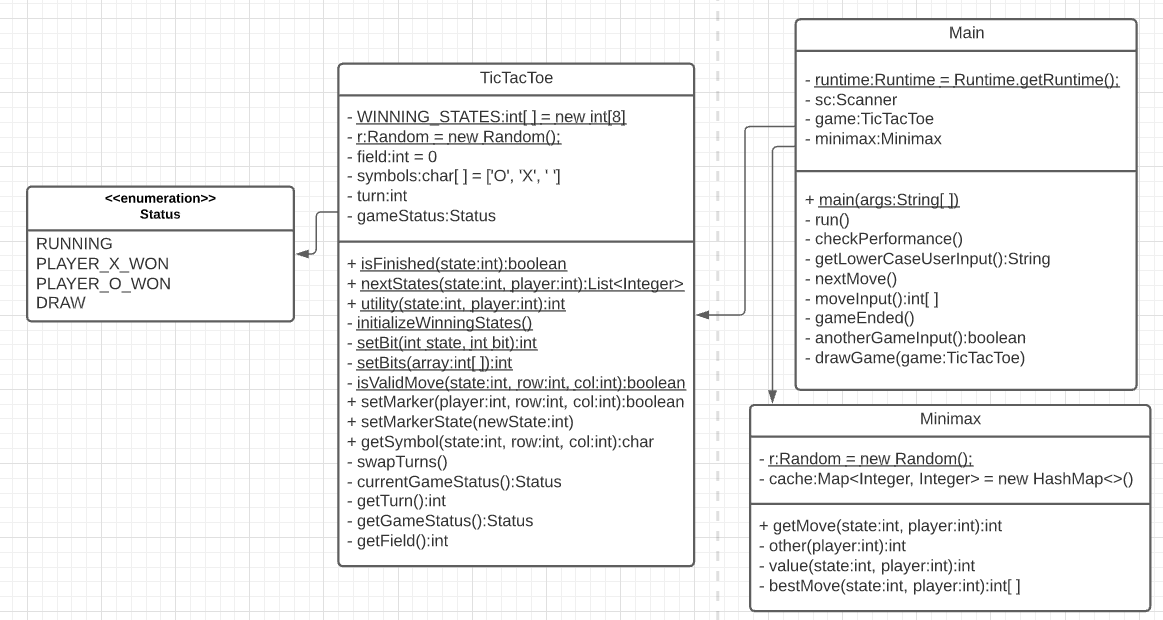
\includegraphics[scale=0.217]{img/uml_diagram.png}
    \caption[Vollständiges Klassendiagramm der Implementierung]{Vollständiges Klassendiagramm der Implementierung (eigene Anfertigung)}
    \label{fig:uml}
\end{figure}

\textbf{Main.java:} Diese Klasse enthält die main-Methode und ist der Startpunkt für das Programm. Sie ist sie dafür
verantwortlich, dass Objekte der anderen beiden Klassen erstellt und verwaltet werden. Die gesamte Logik, welche es ermöglicht, dass 
eine Person eine Runde Tic-Tac-Toe gegen den Minimax-Algorithmus spielen kann, ist in dieser Klasse. Hierzu gehören beispielsweise 
das Abfragen des nächsten Zuges der Person und des Algorithmus sowie alle Ein- und Ausgaben, die zur Bedienung des Programmes notwendig sind. 
Außerdem enthält diese Klasse die Funktion zur Messung der Performance, welche in Kapitel \ref{chap:performancevergleich} zum Einsatz kommt.

\textbf{TicTacToe.java:} Die Klasse TicTacToe ist, wie der Name schon sagt, die Klasse, in der die gesamte benötigte Logik für eine Runde
Tic-Tac-Toe enthalten ist. In dieser Klasse sind sowohl die möglichen Zustände, bei denen ein Spieler das Spiel gewonnen hat als auch der
aktuelle Zustand des Spielbretts gespeichert. Ebenfalls wird der Status des Spiels (siehe enum in Abbildung \ref{fig:uml}) sowie der Spieler, der aktuell
am Zug ist, gespeichert. Des Weiteren sind alle Funktionen enthalten, die zum Anzeigen oder Verändern des Spielfeldes benötigt werden. Hierzu
gehört auch eine Funktion, die ermittelt, ob der gegebene Zug zulässig ist oder das gewünschte Feld bereits belegt ist.

\textbf{Minimax.java:} Innerhalb der Klasse Minimax ist die gesamte Logik für den Minimax Algorithmus enthalten. Hierzu gehören alle Funktionen,
welche benötigt werden, um den bestmöglichen Spielzug bei einem bestimmten Spielstand zu ermitteln. Um alle notwendigen Parameter zu erhalten,
die für die Ermittlung des nächsten Spielzuges benötigt werden, ruft die Klasse Minimax teilweise statische Funktionen der Klasse TicTacToe auf,
welche die notwendigen Werte zurückliefern. Die relevanteste Funktion in dieser Klasse ist die rekursive Funktion \code{value(int state, int player)}, 
da diese in Kapitel \ref{chap:performancevergleich} zur Messung der Performance aufgerufen wird. Die Funktion dient der Bewertung eines möglichen 
Spielzustands anhand der möglichen Gewinnmöglichkeiten (siehe auch Kapitel \ref{chap:minimax}).

\subsection{Performancerelevante Implementierungen im Detail}
\label{chap:implementierungen}
\subsubsection{Spielstand als Bitmaskierung}
Wie fast immer in der Programmierung, gibt es viele verschiedene Möglichkeiten ein Ziel zu erreichen. In diesem Fall ist das Ziel die Speicherung des
Spielstandes, also die Speicherung der Kreuze und Kreise, die bereits gesetzt sind. Möglich wäre hierbei die Speicherung in einer Map, einer Liste, 
einem Feld oder in mehreren Variablen eines geeigneten Datentyps. In diesem Fall wäre womöglich eine Speicherung in einem zweidimensionalen Feld vom Typ
Byte naheliegend. In diesem Feld könnte für jede Koordinate von [0][0] bis [2][2] gespeichert werden, wie der Zustand des entsprechenden Feldes ist (-1 für
leer, 0 für Kreis und 1 für Kreuz). Eine derartige Implementierung würde insgesamt neun Bytes benötigen. Ein Byte für jedes mögliche Feld des Spielbrettes.
Da ein Byte jedoch acht Bits enthält und für die Darstellung von drei Zuständen lediglich 2 Bits benötigt werden, wäre dies eine Verschwendung von Speicherplatz.
Aus diesem Grund wird der gesamte Spielstand in der Implementierung in einem int (4 Bytes) gespeichert. Die ersten neun Bits können gesetzt werden, wenn der erste
Spieler (O) sein Symbol gesetzt hat, während die Bits 9-17 (gezählt ab 0) gesetzt werden, wenn Spieler zwei (X) das Feld gesetzt hat. Die anderen Bits sind nicht
von Relevanz. Der in Abbildung \ref{fig:tictactoestates} gezeigte mögliche zweite Zustand sieht hierbei wie folgt aus:
\begin{figure}[H]
    \centering
    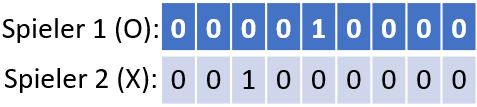
\includegraphics[scale=0.45]{img/bitmaskierung.png}
    \caption[Bitmaskierung eines Tic-Tac-Toe Zustands]{Bitmaskierung eines Tic-Tac-Toe Zustands (eigene Anfertigung)}
\end{figure}
Auf diese Weise können zunächst fünf Byte an Speicher eingespart werden. Ein noch größerer Vorteil ist jedoch der große Performancevorteil, der sich bei dieser
Implementierung ergibt. Da Computer komplett auf dem Binärsystem basieren sind Operationen, welche lediglich einzelne Bits setzen, deutlich schneller als das
Setzen eines ganzes Bytes. Dies hat einen besonders großen Einfluss auf die Laufzeit des Minimax Algorithmus (siehe \ref{chap:minimax}), da dieser immer wieder
rekursiv durch die verschiedenen Zustände rechnen muss und sich deswegen eine Vielzahl an Zugriffen ergeben.


\subsubsection{Caching von Folgezuständen}
Wie in Kapitel \ref{chap:minimax} bereits angedeutet, werden im Laufe eines Tic-Tac-Toe Spiels immer wieder eine große Menge an Folgezuständen geprüft, 
damit der Minimax-Algorithmus in der Lage ist, die verschiedenen bestmöglichen Züge zu ermitteln. Hierbei wird jedem Zustand ein Wert zugeordnet, welcher
anzeigt ob der Zustand im schlechtesten Fall zum Sieg, zum Untenschieden oder zur Niederlage für den Algorithmus führt.
Um zu verhindern, dass die Zustände immer wieder neu auf ihren Wert geprüft werden müssen, wird eine Map<Integer, Integer> erstellt, welche einen
Cache darstellt, der als Schlüssel den Zustand und als Wert den für den Zustand errechneten Wert speichern kann. Jedes Mal, wenn der Wert für einen
möglichen Zustand errechnet werden soll, wird zunächst geschaut, ob dieser Wert bereits im Cache ist. Sollte der Wert sich im Cache befinden, so wird
der Wert aus dem Cache gelesen und weiter verwendet, während im sonstigen Fall einmalig die Berechnung durchgeführt wird. Nach dieser Berechnung wird der 
Wert in den Cache eingetragen, woraufhin der Wert bei zukünftigen Aufrufen nicht jedes Mal neu ermittelt werden muss.

\section{Performancevergleich von Java und Python}
\label{chap:performancevergleich}

Nachdem der Minimax-Algorithmus für das Spiel Tic-Tac-Toe in Java implementiert wurde, soll nun die 
Performance mit der Umsetzung in Python verglichen werden. Hierfür wird bei beiden Versionen die Funktion 
\code{value} für ein leeres Spielfeld mit Spieler 0 aufgerufen. D. h. die Funktion \code{value} berechnet 
alle möglichen Spielzustände und deren Wert. Die CPU-Zeiten beziehen sich auf eine Testreihe mit einem 
Intel i7-9700K. Für jeden Test werden jeweils fünf Durchgänge mit und ohne Memoisierung durchgeführt 
und daraus der Durchschnittswert berechnet.

\begin{table}[H]
    \centering
    \begin{tabular}{|l|ll|l|}
        \hline
        \multicolumn{4}{|l|}{\textbf{RAM}}                                             \\ \hline
                                & ohne memoize & mit memoize &                         \\ \hline
        \multirow{1}{*}{Python} &              & 808         & \multirow{7}{*}{in KB}  \\ \cline{1-3}
        \multirow{5}{*}{Java}   & 12875        & 1515        &                         \\
                                & 13392        & 1515        &                         \\
                                & 13387        & 1515        &                         \\
                                & 12881        & 1515        &                         \\
                                & 13391        & 1514        &                         \\ \cline{1-3}
        average                 & 13185,2      & 1514,8      &                         \\ \hline
    \end{tabular}
    \caption{Ergebnisse der Performancetestreihe für den genutzten Arbeitsspeicher}
\end{table}

Da für den belegten Arbeitsspeicher der Python Implementierung keine verlässlichen Messwerte gemessen werden 
konnten, wird der Messwert aus dem Jupyter-Notebook (Bitboard mit Memoisierung) verwendet. Auffallend ist, 
dass die Java Implementierung selbst mit Memoisierung, fast doppelt so viel Speicher verbraucht wird. 
Darüber hinaus kann durch Memoisierung bei der Implementierung in Java der Speicherverbrauch um den 
Faktor 8,5 reduziert werden.

\begin{table}[H]
    \centering
    \begin{tabular}{|l|ll|l|}
        \hline
        \multicolumn{4}{|l|}{\textbf{CPU Time}}                                        \\ \hline
                                & ohne memoize & mit memoize &                         \\ \hline
        \multirow{5}{*}{Python} & 2520         & 42,6        & \multirow{12}{*}{in ms} \\
                                & 2520         & 45          &                         \\
                                & 2520         & 44          &                         \\
                                & 2510         & 42          &                         \\
                                & 2510         & 44          &                         \\ \cline{1-3}
        average                 & 2516         & 43,92       &                         \\ \cline{1-3}
        \multirow{5}{*}{Java}   & 43           & 8           &                         \\
                                & 43           & 8           &                         \\
                                & 44           & 9           &                         \\
                                & 45           & 7           &                         \\
                                & 42           & 8           &                         \\ \cline{1-3}
        average                 & 43,4         & 8           &                         \\ \hline
    \end{tabular}
    \caption{Ergebnisse der Performancetestreihe für die benötigte Zeit}
\end{table}

Die Schnelligkeit der Python-Implementierung mit Memoisierung ist in etwa gleich zur Java-Implementierung 
ohne Memoisierung. Mit Memoisierung kann die Laufzeit durch die Verwendung von Java nochmal um 80\% verringert 
werden.

\section{Java vs. Python}
Neben den in Kapitel \ref{chap:implementierungen} gezeigten Unterschieden bei der Implementierung, können die in Kapitel 
\ref{chap:performancevergleich} ermittelten Performanceunterschiede durch Unterschiede in der Funktionsweise der 
Sprachen erklärt werden.

\subsection{Memory Management}
Während Python oft als unperformant wahrgenommen wird, konnte Python beim Arbeitsspeicherverbrauch im Vergleich 
zu Java punkten. Dies kann vorallem durch Unterschiede beim Speichermanagement der beiden Sprachen erklärt werden. 

Arbeitsspeicher wird in Python über einen Heap, der intern verwaltet wird. Wird also Arbeitsspeicher benötigt, 
wird dieser durch das Memory-Management vom Betriebssystem angefordert. Objekte bleiben nur so lange im Speicher 
wie sie benötigt werden. Python nutzt das sogenannte Reference Counting um Objekte zu speichern.

\begin{lstlisting}[caption={Codebeispiel zur Verwaltung von Objekten in Python}]
    a = 9
    b = 9
    c = 11
\end{lstlisting}

In diesem Beispiel wird der Wert 9 als Objekt im Speicher erstellt und Variable \code{a} zugewiesen. Da 
Das Objekt mit dem Wert 9 schon existiert, wir Variable {b} als weitere Referenz hinzugefügt. Für Variabl 
\code{c} heißt das, dass ein Objekt mit dem Wert 11 angelegt werden muss und \code{c} als Referenz hinterlegt wird. 
Beträgt die Anzahl der Referenzen eines Objekts Null, so wird es aus den Speicher entfernt. Die Referenzen 
werden zyklisch vom Garbage Collector überprüft und Objekte ohne Referenzen entfernt. Reference Counting 
hat den Vorteil, dass nicht genutzter Speicher sehr schnell erkannt wird. Allerdings entsteht durch das Zählen 
der Referenzen ein gewisser Overhead, der im Vergleich zu anderen Garbage Collecting Verfahren aber eher gering ausfällt.

%TODO: Garbage Collection Java